\documentclass[9pt,a4paper]{report}
\usepackage{mwe}
\usepackage{listings}
\usepackage{amsmath}
\usepackage{graphicx}
\usepackage{subfig}
\usepackage{float}
\usepackage{xcolor}
\usepackage{multirow}
\usepackage{hyperref}
\usepackage{fancyhdr}
\usepackage{sectsty}
\usepackage[dvipsnames]{xcolor}
\usepackage{soul}
\usepackage[compact]{titlesec}
\usepackage{float}
\usepackage[left=0.5cm,right=0.5cm,top=0.5cm,bottom=0.5cm]{geometry}
\graphicspath{{Parallel Opposing Polarities Diode Circuit}{Series Opposing Polarities Zener Diode Circuit}}

\newcommand*{\nchapter}[1]{%
	\chapter*{#1}%
	\addcontentsline{toc}{chapter}{#1}
	\vspace{-14mm}}
\newcommand*{\nsection}[1]{%
	\section*{#1}%
	\addcontentsline{toc}{section}{#1}}
\newcommand*{\nsubsection}[1]{%
	\subsection*{#1}%
	\addcontentsline{toc}{subsection}{#1}}
\newcommand*{\nsubsubsection}[1]{%
	\subsubsection*{#1}%
	\addcontentsline{toc}{subsubsection}{#1}}

\chaptertitlefont{\large}
\sectionfont{\normalsize}
\fontsize{9}{11}\selectfont
\begin{document}
	\begin{titlepage}
		\centering
		\vspace*{1.5in}
		
\includegraphics[width=0.15\textwidth]{W-Logo_Purple_RGB}\par\vspace{1cm}
		{\LARGE \textsc{University of Washington}\par}
		\vspace{1cm}
		{\Large \textsc{BEE331 Lab 1.3}\par}
		\vspace{1.5cm}
		{\huge\bfseries \par}
		\vspace{2cm}
		{\Large\itshape 2301991\hspace{55pt}1900585\par}
		{\Large\itshape Jason Truong\hspace{31pt}Henry Haight\par}
		\vfill
		supervised by\par
		Prof.~Joseph \textsc{Decuir}
		\date{2024\\ January}
		\vfill
		% Bottom of the page
		{\large \today\par}
		\vspace*{1.5in}
	\end{titlepage}
	
	\nchapter{Voltage Limiter Circuits; Standard \& Zener Diode}
	\nsection{Design Objective}
	In this lab, we introduce ourselves to two voltage-limiting circuits. One built with standard diodes and the other built with Zener diodes., we characterise its function by the I-V curve.
	\begingroup
	\renewcommand{\cleardoublepage}{}
	\renewcommand{\clearpage}{}
	\nsection{Circuit Design Outline}
	\endgroup
	With a resistor of an arbitrary impedance greater than $100\Omega$ ($R\geq100\Omega$), and the natural impedance of the Function Generator in series ($R_{TOT}=R_{FG}+R\geq150\Omega$), the designed High-Level Limiter Circuit is set in series to the resistor; through the function generator. Set the function generator @ f=200kHz and $V_P=5V,0.1V,10V$ in High-Z impedance.
	\begin{figure}[h!]
		\centering
		\caption{\centering High-Level Limiter Circuit}
		\subfloat[\centering Rudimentary Generic Schematic of High-level Limiter Circuit]{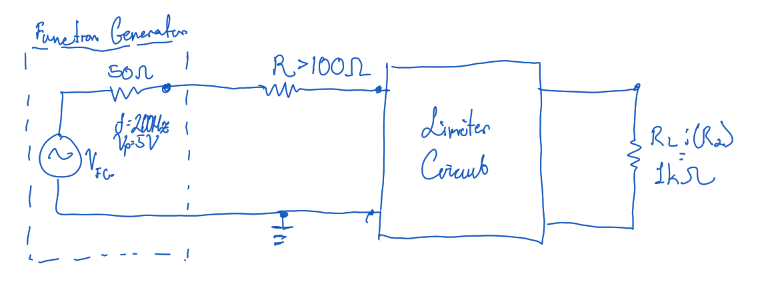
\includegraphics[width=19cm]{Screenshot 2024-07-15 211530}}
	\end{figure}
	\begin{figure}[h!]
		\ContinuedFloat
		\centering
		\subfloat[\centering LTSpice + Rudimentary Schematic Parallel Standard Diodes Circuit]{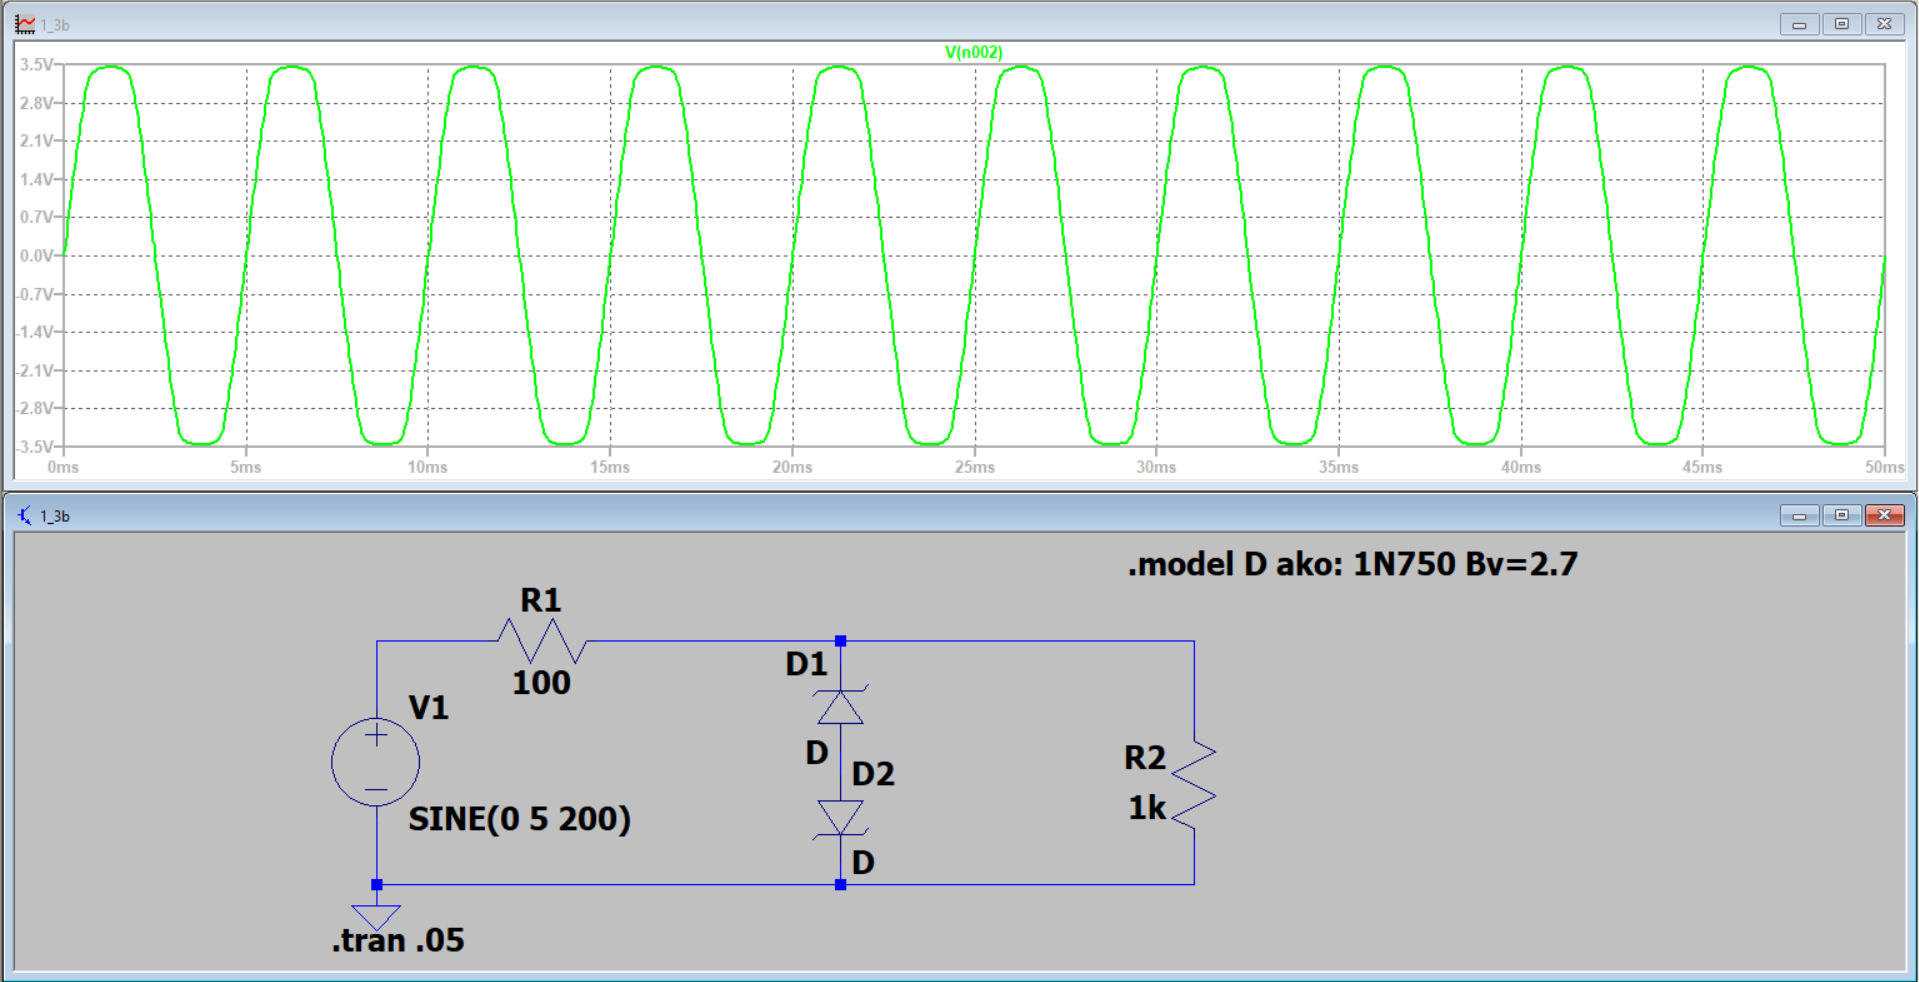
\includegraphics[width=9cm]{Screenshot 2024-07-15 063021}}
		\subfloat[\centering LTSpice + Rudimentary Schematic Series Opposing Zener Diodes Circuit]{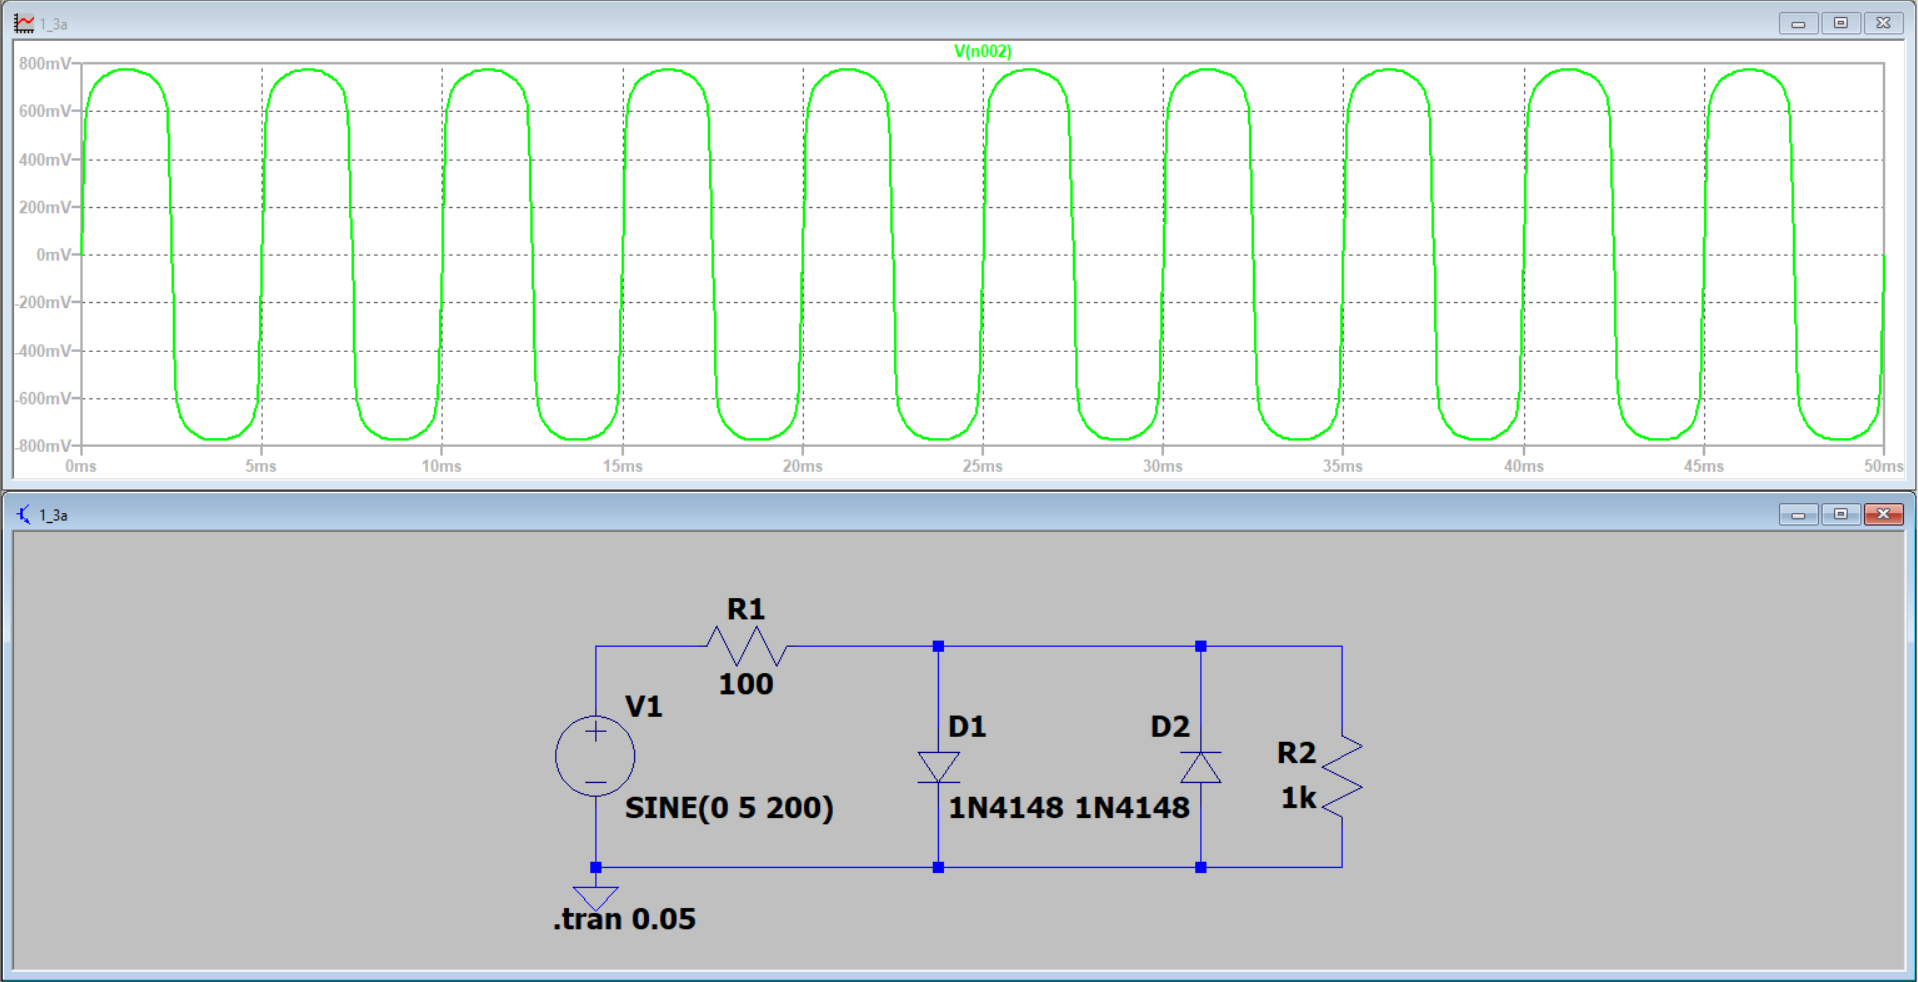
\includegraphics[width=9cm]{Screenshot 2024-07-15 063246}}
	\end{figure}
	\begin{figure}[h!]
		\ContinuedFloat
		\centering
		\subfloat[\centering Parallel Standard Diodes Circuit]{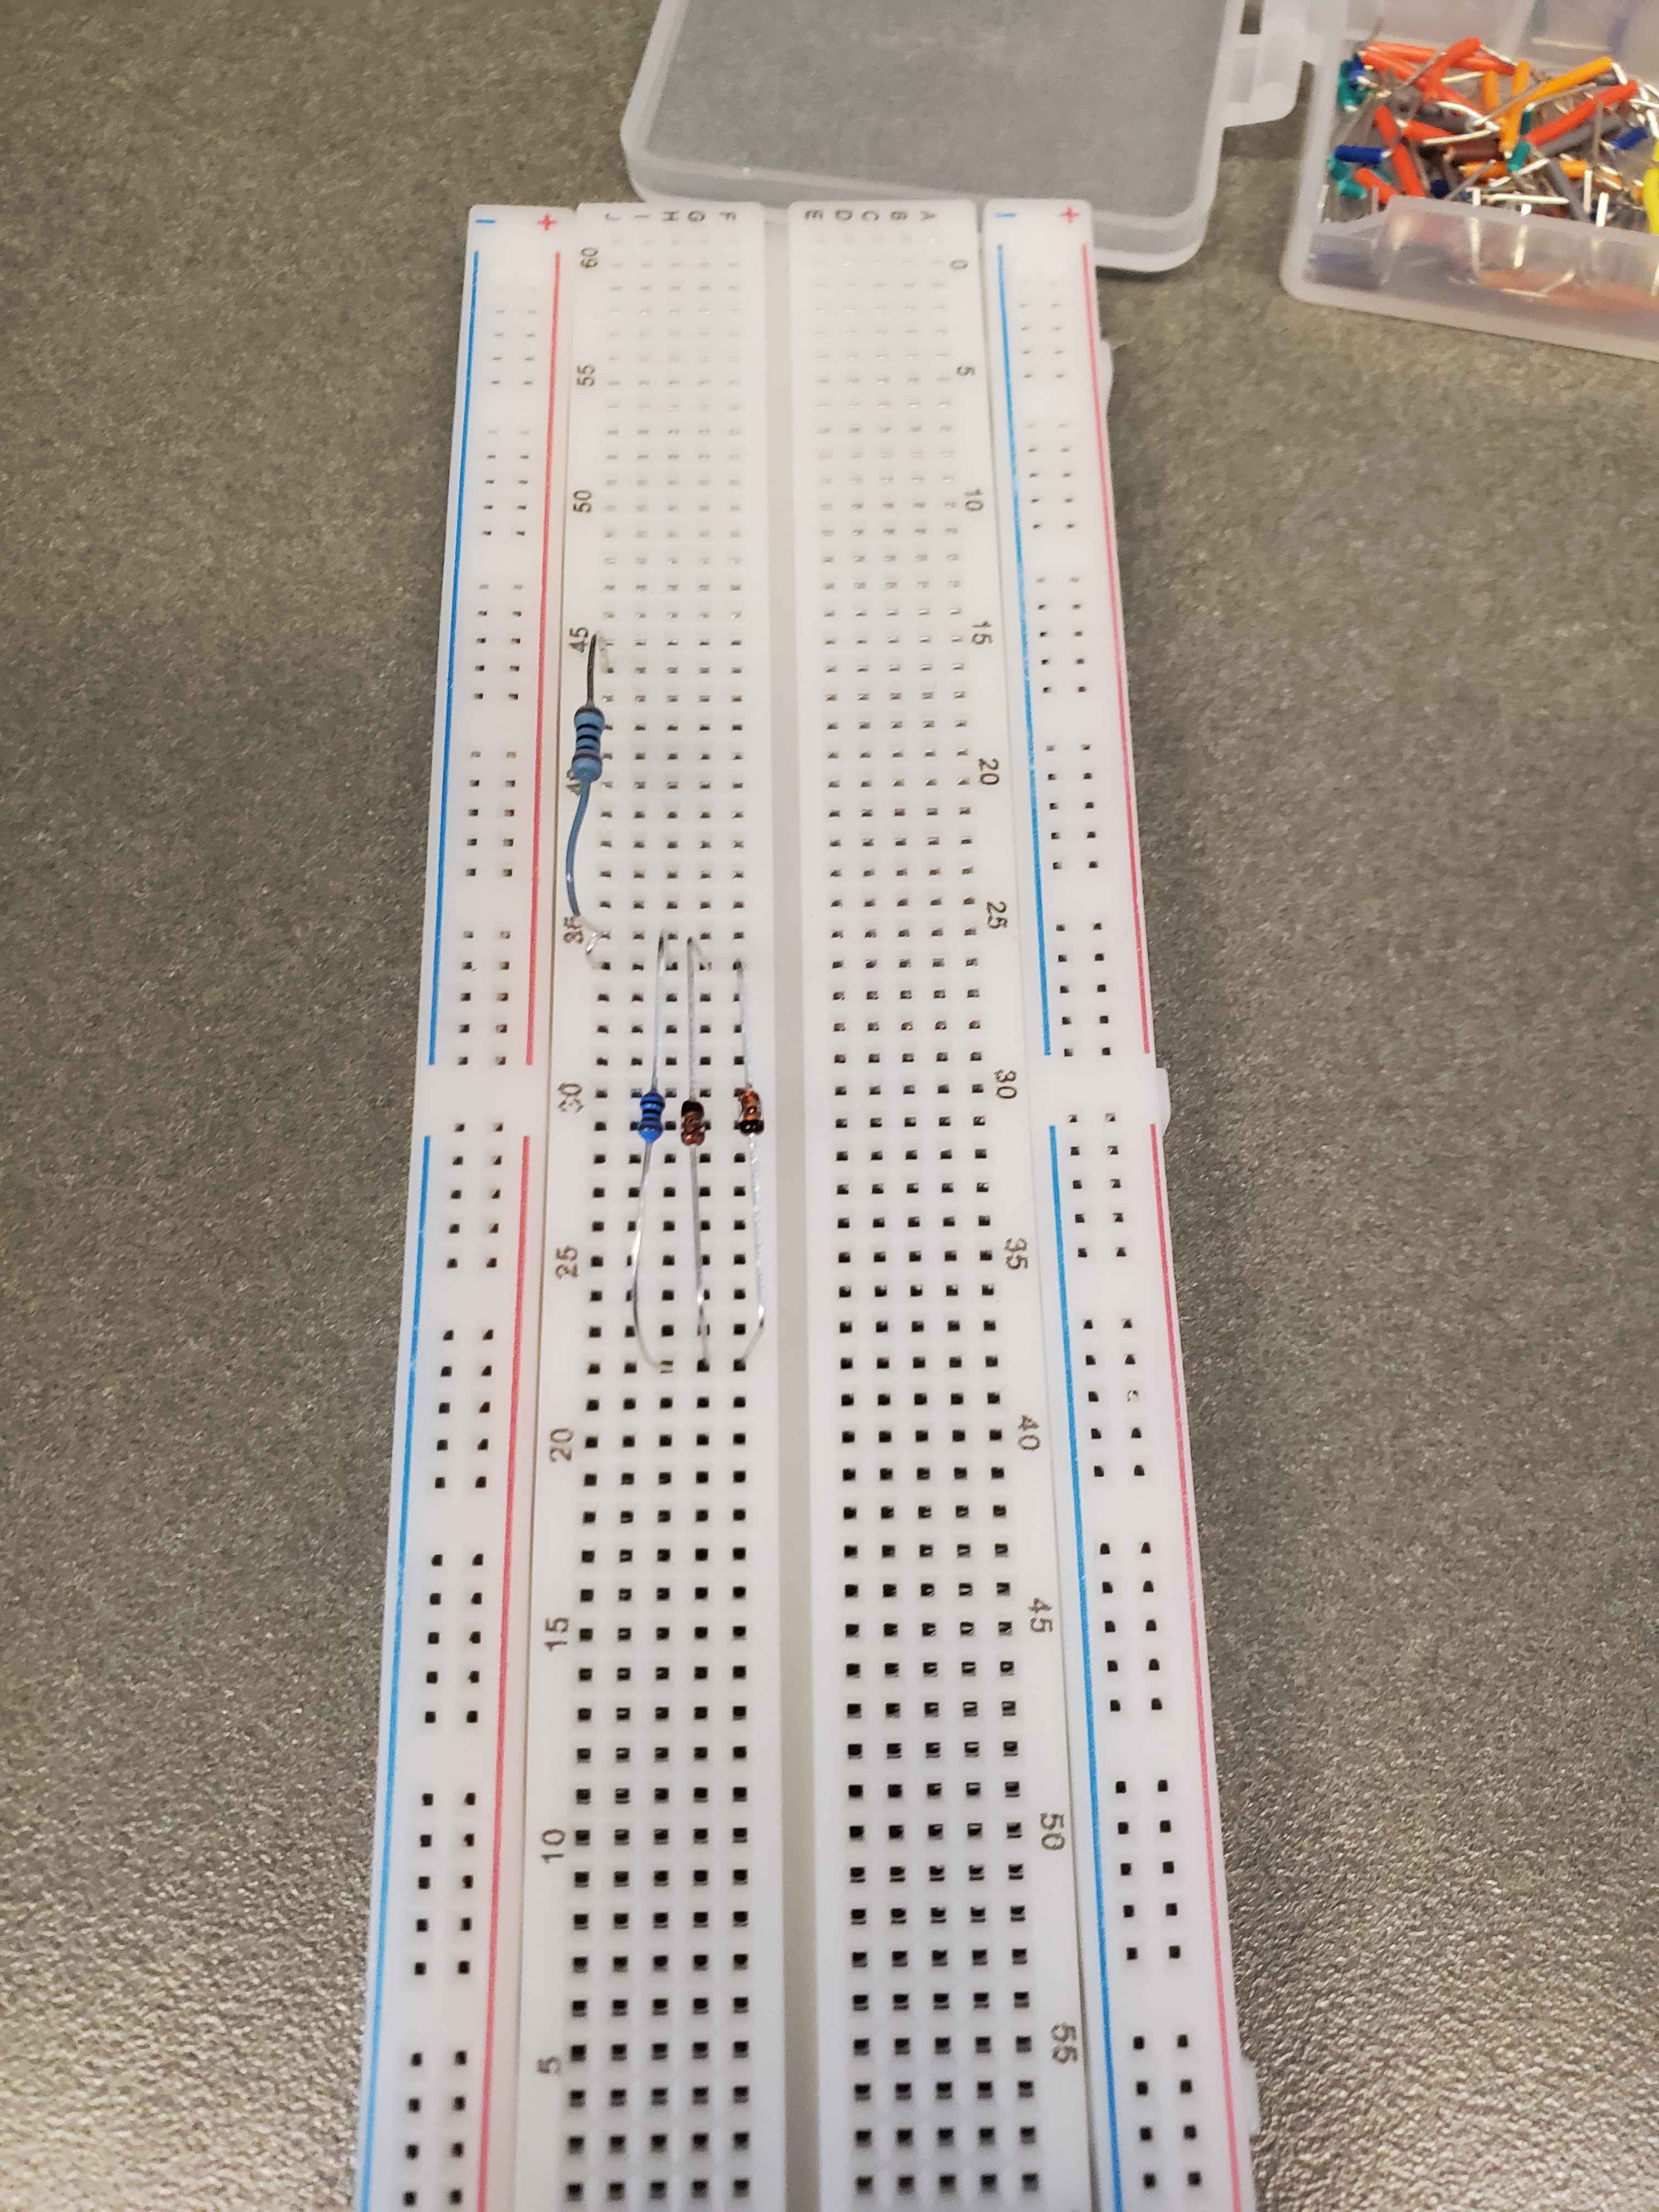
\includegraphics[width=9cm]{20240703_124842}}\hfil
		\subfloat[\centering Series Opposing Zener Diodes Circuit]{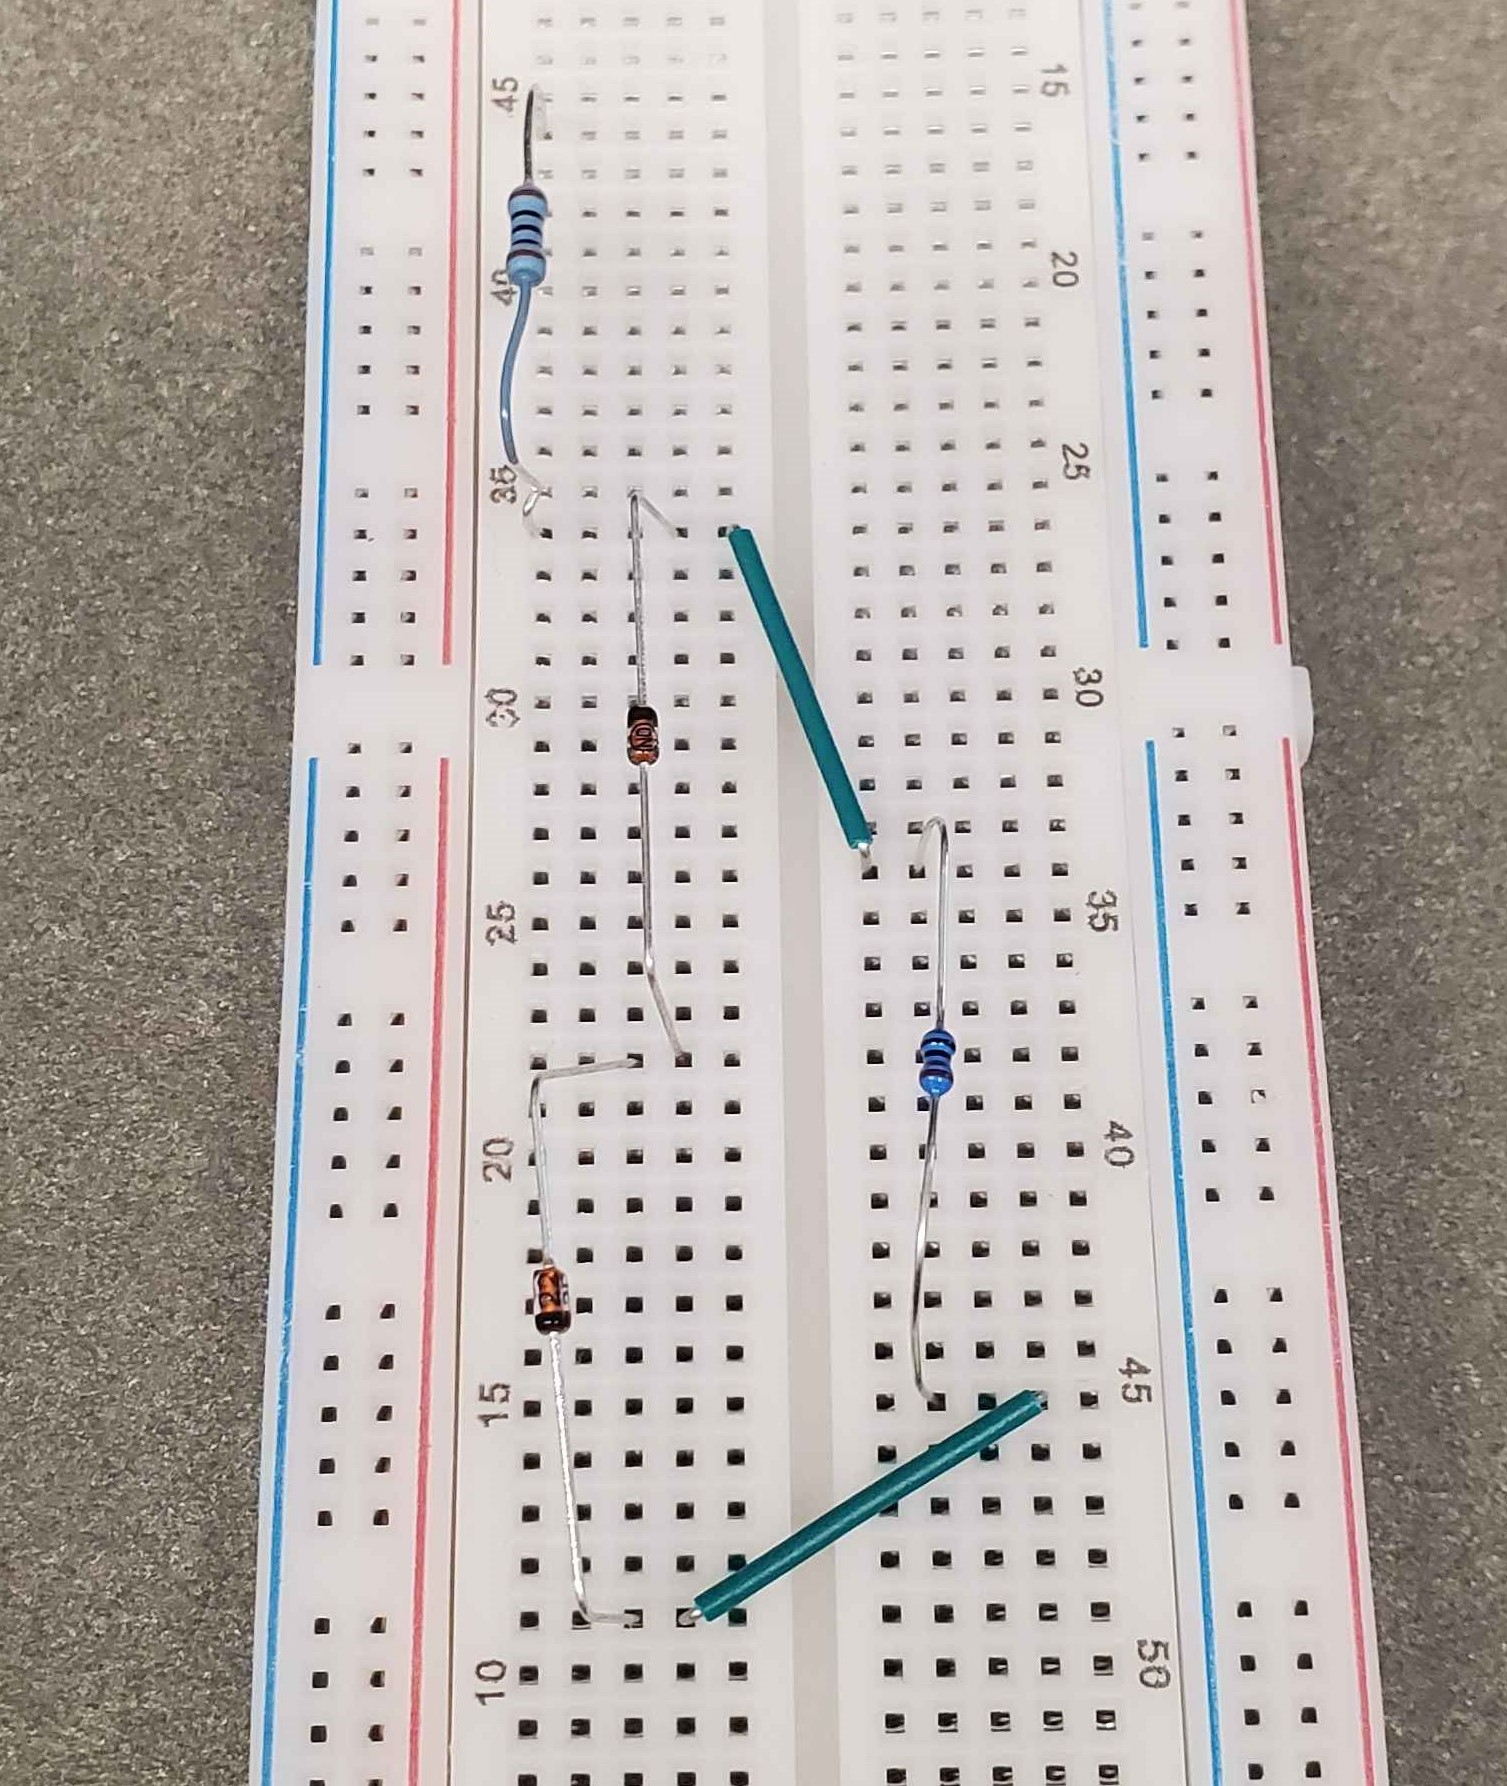
\includegraphics[width=9cm]{20240703_124754}}
	\end{figure}
	
	\newpage
	
	\nsection{Descriptions of Measurements \& Calculations}
	Given the default theoretical calculation for a Diode in forward-bias: $I_D=I_S(e^{\frac{V_D}{V_T}}-1)$; the dataset is similar in-nature - not exact because the characteristics of this diode differs - from section 1.1 of the lab.\\
	The characteristic of a \textit{Zener} Diode is its relationship to $-V_D$, as $I_D$ enters \textbf{Reverse-Breakdown} @ $-V_{Z0}$; the point of breakdown.\\
	Because of these characteristics, the Limiter-Circuits meet their respective "off" thresholds to logarithmically degrade the output voltage of $V_o$.
	\begin{figure}[h!] %140, 
		\centering
		\caption{High-Limiter Circuit Scope}
		\subfloat[Parallel RDD Circuit @ $0.1V_p$]{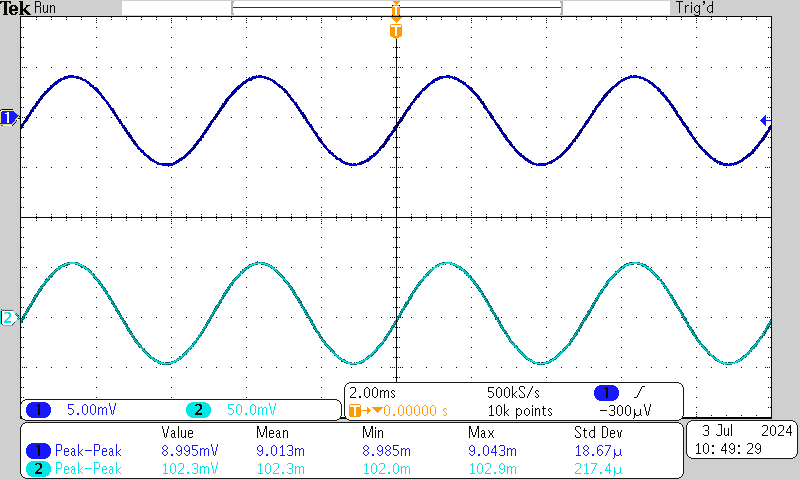
\includegraphics[width=8cm]{tek0000}}\hfil
		\subfloat[Parallel RDD Circuit @ $10V_p$]{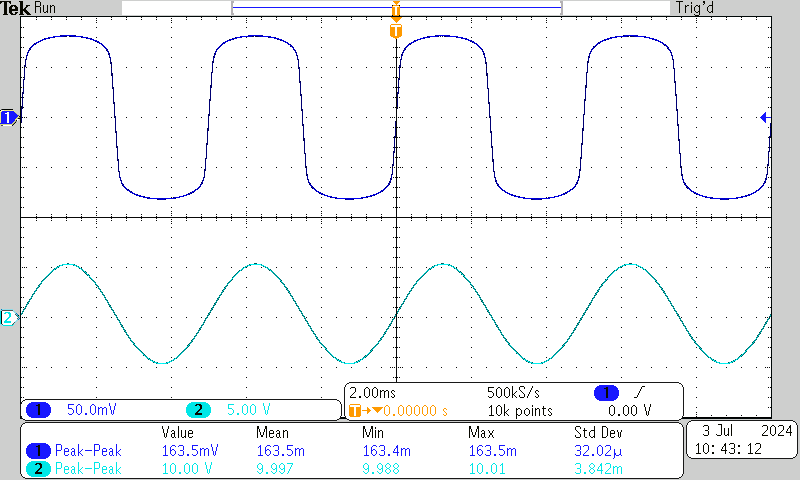
\includegraphics[width=8cm]{tek0001}}\hfil
		\subfloat[Series Opposing-Polarity Zener Diode Circuit @ $0.1V_p$]{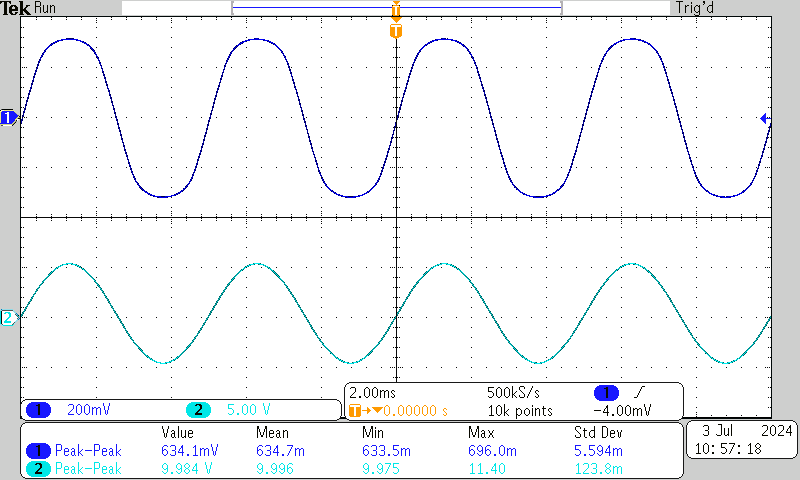
\includegraphics[width=8cm]{tek000000}}\hfil
		\subfloat[Series Opposing-Polarity Zener Diode Circuit @ $10V_p$]{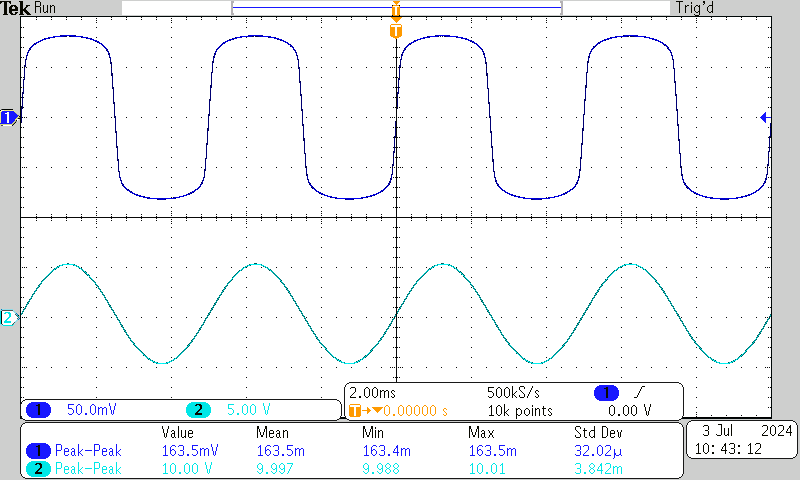
\includegraphics[width=8cm]{tek0001}}
	\end{figure}
	\nsection{Summary \& Conclusions}
	Revealed in Figure RDD-Circuit 0A \& 0B, the generated oscilloscope readings of the two periodic function do in-fact dampen @ $V_{in}$ (CH2) greatly to $V_{out}$ (CH1). It is similary in the Series $D_Z$ circuit.
	\nsubsection{Discussion}
	\begin{itemize}
		\item \textbf{i. Describe how each limiter circuit limits the input voltage based on the output waveform you measured. How are the limiter circuits 1 and 2 different?}
		\subitem The first limiter circuit reduces peak voltage showing the behavior of the exponential diodes. This makes the output wave more square than the input wave because it is limiting the input before it can start curving back down. [Reference Above]
		\item \textbf{ii. What is the effect of setting the \textit{Load Impedance to High Z} mode for the function generator?}
		\subitem \emph{Forward-Bias:} $I_D=I_S(e^{\frac{V_D}{V_T}}-1)$; reference Figure 1b.
		\subitem The instrument will display less attenuation when producing the signal; so in ley, less of a impeded signal.
		\item \textbf{iii. What settings did you use in the oscilloscope in order to suppress noises in the output signals??}
		\subitem \emph{Forward-Bias:} The characteristics of the I-V curve of a diode has current $I_D$ exponentially rise towards a cut-off at the threshold, towards the C.V.D @ $V_D$.
		\subitem High-Fine, Auto-range, 50\% auto-trigger, AC-Coupling.
		\item \textbf{iv. For the limiter Circuit 1, can you make the output signal the same as the input signal by changing $v_{peak}$}
		\subitem You should be able to make the output signal the same by staying in the region where both diodes are in an "off" state. This will cause the circuit to not be limited by current through the diodes.
	\end{itemize}
	\newpage
	\newpage
	\nsection{Bibliography}
	\textbf{Cited:}\\
	\begin{itemize}
		\item Lab 1 Manual
		\item Sedra, Adel, and Kenneth Smith. Microelectronic Circuits. S.L., Oxford Univ Press Us, 2019.
		\item “How Do You Calculate, a Silicon Junction Diode with N = 1 Has v = 0.7 v al I = 1 MA. What Is the Voltage Drop at I=0.1 MA and I=10 MA.?” Quora, 2024, appliedmathematics.quora.com/How-to-calculate-A-silicon-junction-diode-with-n-1-has-v-0-7-V-al-I-1-mA-What-is-the-voltage-drop-at-I-0-1-mA-an?top\_ans=223007030. Accessed 15 July 2024.
	\end{itemize}
	\begin{figure}[!h]
		\subfloat[Look at her, she's perfect.]{
\includegraphics[width=\linewidth]{GodILoveFurina}}
	\end{figure}
\end{document}